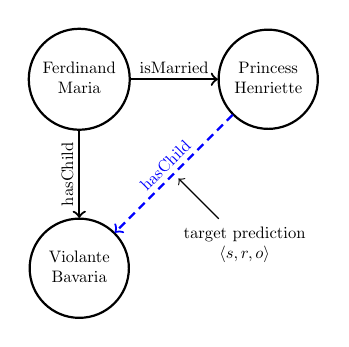
\begin{tikzpicture}[scale=0.6, every node/.style={scale=0.6}]
\node[draw,circle,thick,inner sep=0,minimum size=2.1cm] (o_fm) at (0,0) {\begin{tabular}{c} Ferdinand \\ Maria \end{tabular}};
\node[draw,circle,thick,inner sep=0,minimum size=2.1cm] (o_ph) at (4,0) {\begin{tabular}{c} Princess\\ Henriette\end{tabular}};
\node[draw,circle,thick,inner sep=0,minimum size=2.1cm] (o_vb) at (0,-4) {\begin{tabular}{c} Violante\\ Bavaria\end{tabular}};
\draw[->,thick] (o_fm) -- (o_ph) node[pos=0.5, sloped,align=center, above]{isMarried};
\draw[->,thick] (o_fm) -- (o_vb) node[pos=0.5, sloped,align=center,rotate=180, above]{hasChild};
\draw[->,thick,blue,densely dashed] (o_ph) -- (o_vb) node[pos=0.5, sloped,align=center, above] {hasChild};
\node (a) at (3.5,-3.5) {\begin{tabular}{c} target prediction\\ $\langle s,r,o\rangle$\end{tabular} };
\draw[->] (a) -- (2.1,-2.1);
\end{tikzpicture}